\documentclass[12pt,a4paper]{article}

% Packages utiles
\usepackage[utf8]{inputenc}
\usepackage{amsmath, amssymb}
\usepackage{graphicx}
\usepackage{booktabs}
\usepackage{hyperref}
\usepackage{subcaption}
\usepackage{tabularx}
\usepackage{array}
\usepackage{booktabs}
\usepackage{siunitx}
\usepackage{makecell} % for multi-line headers
\sisetup{
  group-separator = {\,},
  input-ignore = {,},
  detect-all,
}
% Column helpers
\newcolumntype{L}[1]{>{\raggedright\arraybackslash}p{#1}} % fixed-width, left
\newcolumntype{Y}{>{\raggedright\arraybackslash}X}        % auto-width, left

\title{Dose–Response Meta-Analysis of Adverse Events in Psychedelic Studies}
\author{Mickael Eskinazi, Michel Sabe}
\date{\today}

\begin{document}

\maketitle

\begin{abstract}

\end{abstract}

\section{Introduction}


\section{Methods}

\subsection{Data sources and study selection}
We compiled data from randomized controlled trials and prospective studies reporting adverse events (AEs) in the context of psychedelic administration (LSD, psilocybin, MDMA, and ayahuasca). Studies were included if dosing arms were clearly specified and adverse events were systematically recorded. Animal studies, case reports, and trials lacking structured AE reporting were excluded.  

Study information was extracted into a structured dataset, including identifiers, treatment arms, dose levels, time windows (acute session vs. follow-up), and AE terms. A total of 17 studies were retained, covering four molecules with diverse dose ranges and control conditions (Table~\ref{tab:study_summary}).  

\subsection{Data extraction and harmonization}
For each study arm, we extracted:  
(i) molecule and dose (in mg or mg/kg),  
(ii) participant count,  
(iii) type of control condition (inactive or active placebo),  
(iv) reported AE terms.  

AE terms were harmonized manually across studies to reduce redundancy (e.g., “GI symptoms” vs. “abdominal pain,” “visual perceptual effects” vs. “illusions”). Each AE was coded as binary (present/absent per participant). The variable \texttt{arm\_id} was mapped into dose categories (placebo, low, mild, high).  

\subsection{Control conditions}
Control arms varied across molecules, including both inactive placebos (e.g., saline, mannitol) and active placebos (e.g., niacin, very-low-dose LSD). Inactive placebos were considered reference when available; otherwise, active placebos were used; if no control was reported, dose–dose contrasts within a study were employed. Table~\ref{tab:placebo_types} summarizes the distribution of control conditions by molecule.  

\subsection{Statistical analysis}
Pairwise contrasts were computed by aligning each active arm with an appropriate control condition (inactive or active placebo). When no placebo was available, contrasts were constructed using dose-difference between study arms.  

Adverse event incidence rates were transformed into log-odds ratios (log(OR)) using the \texttt{metafor} package in R. Random-effects meta-analyses (restricted maximum likelihood, REML) were conducted for each AE.  

Dose–response relationships were modeled using restricted cubic splines (\texttt{rms} and \texttt{dosresmeta} packages), with study-level random effects. We generated dose–response curves overall (all AEs pooled) and stratified by molecule, as well as facet plots for individual AEs. When multiple molecules reported the same AE, dose–response curves were overlaid for cross-molecule comparison.  

Forest plots were also constructed, pooling across studies for each AE and stratified by molecule. Statistical significance was defined as $p<0.05$ for non-intercept dose terms. Significance was visualized with stars ($^{*}p<0.05$, $^{**}p<0.01$, $^{***}p<0.001$), shown directly on dose–response curves and forest plots.  

\subsection{Software and reproducibility}
All analyses were performed in R (version 4.3.2) using the following packages: \texttt{tidyverse}, \texttt{metafor}, \texttt{dosresmeta}, \texttt{splines}, \texttt{patchwork}, and \texttt{ggplot2}.  
The full analysis pipeline, including scripts for data harmonization and figure generation (\texttt{analysis\_plots\_master.R}), is available at:  
\url{https://github.com/mickaeleskinazi/metaanalysis-psychedelics}.  

\subsection{Summary of dataset}
As shown in Table~\ref{tab:study_summary}, the final dataset included 17 studies overall, covering four molecules with diverse dose ranges and control conditions. Psilocybin studies contributed the largest number of unique AE terms ($n=99$), followed by LSD ($n=43$), MDMA ($n=26$), and ayahuasca ($n=12$). This heterogeneity illustrates differences in reporting practices and provides an opportunity to assess cross-molecule patterns in AE occurrence.  

\begin{table}[htb]
\centering
\small
\setlength{\tabcolsep}{4pt}
\renewcommand{\arraystretch}{1.15}
\caption{\textit{Summary of included studies by molecule: cleaned dose range (mg), placebo type(s), number of studies, total participants, and vocabulary richness (unique AE terms). Placebo arms (0 mg) excluded from dose ranges.}}
\label{tab:study-summary}
\begin{tabularx}{\textwidth}{@{} l l L{3.0cm} S[table-format=2.0] S[table-format=3.0] S[table-format=3.0] @{}}
\toprule
\textbf{Molecule} & \textbf{Dose(mg)} & \makecell[l]{\textbf{Placebo}\\\textbf{type(s)}} & {\textbf{Studies}} & {\textbf{Participants}} & {\textbf{AE terms}} \\
\midrule
Ayahuasca  & 0.36--0.36 & Active           & 2  & 24  & 12 \\
LSD        & 0.02--200  & Inactive, Active & 6  & 234 & 72 \\
MDMA       & 25--150    & Active           & 10 & 215 & 26 \\
Psilocybin & 1--40      & Active           & 8  & 300 & 96 \\
\bottomrule
\end{tabularx}
\end{table}

\begin{table}[htb]
\centering
\caption{\textit{Distribution of placebo conditions across molecules. Values represent number of studies including each type of placebo.}}
\label{tab:placebo-distribution}
\begin{tabular}{lcc}
\toprule
Molecule & Inactive placebo & Active placebo \\
\midrule
Ayahuasca & 0 & 2 \\
LSD       & 1 & 3 \\
MDMA      & 0 & 10 \\
Psilocybin& 0 & 8 \\
\bottomrule
\end{tabular}
\end{table}


\section{Results}

\subsection{Overview}
We analyzed dose--response (DR) relationships and pooled odds ratios (OR) for adverse events (AEs) across four molecules (LSD, MDMA, psilocybin, ayahuasca), and across two time windows: \emph{session} (acute) and \emph{follow--up}. We first report global DR patterns by molecule (all AEs pooled), then AE-specific DR overlays (same AE across multiple molecules), and finally pooled forest summaries by molecule. We close this section with a direct comparison of \emph{session} vs \emph{follow--up} significance patterns using the publication tables.

\subsection{Global dose--response trends by molecule (all AEs pooled)}
All three main molecules (LSD, MDMA, psilocybin) showed a significant overall dose effect on AE incidence (global tests $p<0.001$ for each; Table~\ref{tab:global}). MDMA displayed a roughly monotonic increase of AE risk with dose; LSD and psilocybin showed non-linear (spline) shapes where mid-range doses are somewhat better tolerated than very low or very high doses. These global relationships are visualized in Figure~\ref{fig:dr_global}, which expresses log(OR) vs.\ dose (molecule-specific scaling) with 95\% CIs.

\begin{figure}[htb]
  \centering
  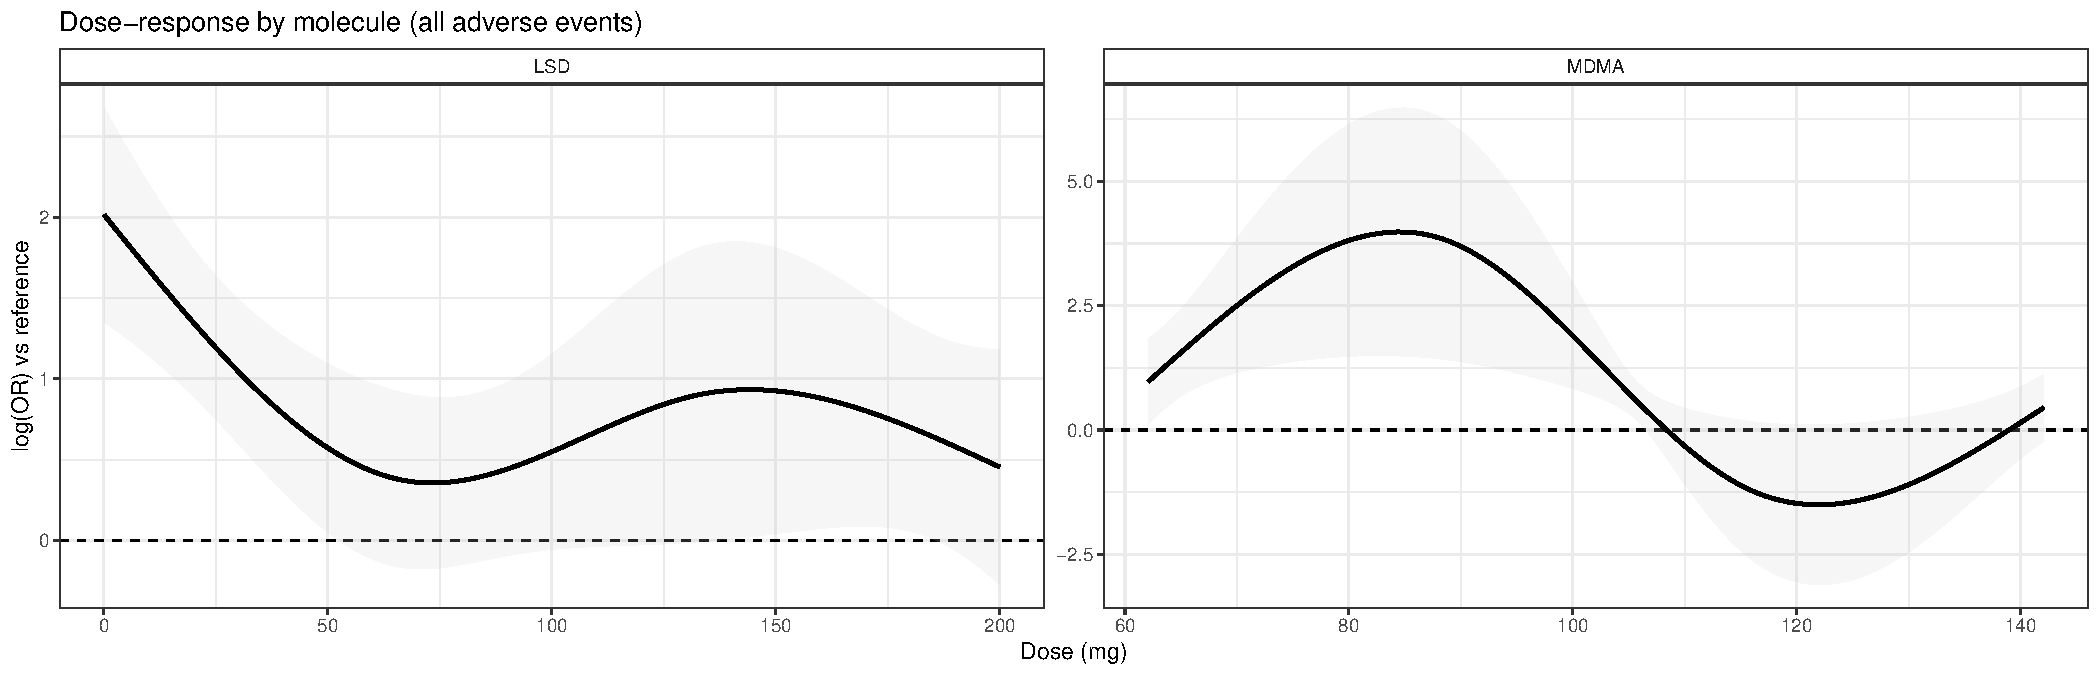
\includegraphics[width=0.95\textwidth]{master_dr_by_molecule.pdf}
  \caption{\textit{Global dose--response curves for adverse events across LSD, MDMA, and psilocybin. The $y$--axis shows log(OR) vs.\ reference. Shaded bands: 95\% CIs. MDMA increases approximately linearly; LSD and psilocybin show non-linear patterns.}}
  \label{fig:dr_global}
\end{figure}

\begin{table}[htb]
\centering
\caption{\textit{Overall dose--response test results by molecule. $Q_M$ is the omnibus test for dose as moderator; $p_{\text{overall}}$ is the global dose effect.}}
\label{tab:global}
\begin{tabular}{lcccc}
\toprule
Molecule & Total $k$ & $Q_M$ & $p_{\text{overall}}$ & Significance \\
\midrule
LSD        & 292 & 2.93  & $1.13\times 10^{-5}$  & *** \\
MDMA       & 218 & 15.85 & $1.72\times 10^{-11}$ & *** \\
Psilocybin & 162 & 19.13 & $3.94\times 10^{-11}$ & *** \\
\bottomrule
\end{tabular}
\end{table}

\subsection{AE-specific dose--response overlays (cross-molecule)}
To identify which AEs are dose-sensitive and how profiles differ by molecule, we generated overlays for AEs observed in at least two molecules, with model-based DR curves and significance stars (on-curve) for non-intercept dose terms ($^{*}p<0.05$, $^{**}p<0.01$, $^{***}p<0.001$). Representative panels are shown in Figure~\ref{fig:dr_overlays_panels}; the full grid and per-AE PDFs are provided in Supplementary Figures.

\begin{figure}[htb]
  \centering
  \begin{subfigure}{0.32\textwidth}
    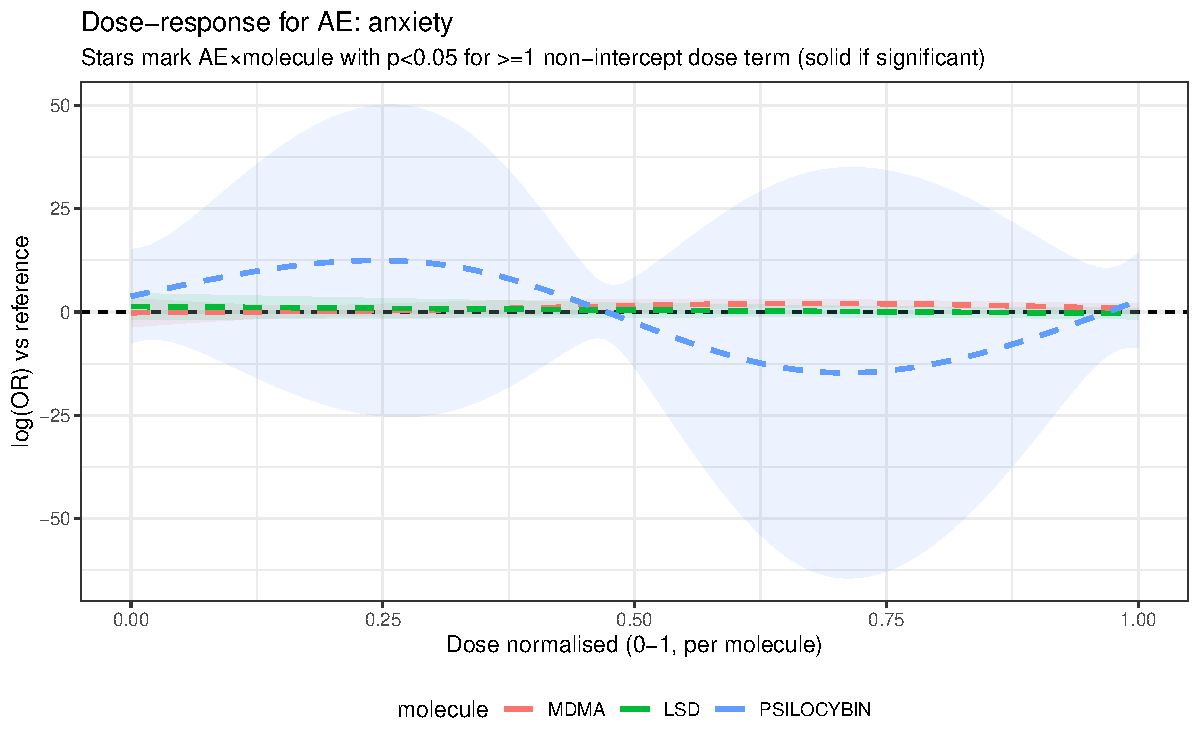
\includegraphics[width=\linewidth]{DR_overlay_anxiety.pdf}
    \caption{Anxiety}
  \end{subfigure}\hfill
  \begin{subfigure}{0.32\textwidth}
    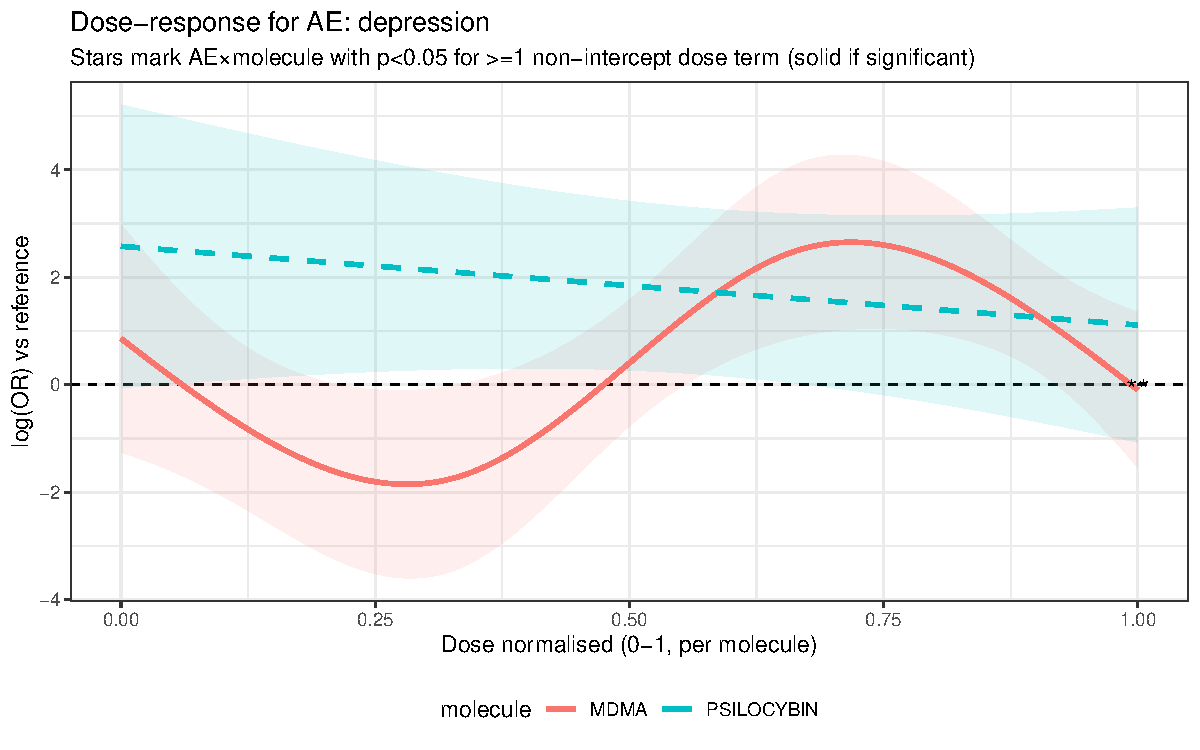
\includegraphics[width=\linewidth]{DR_overlay_depression.pdf}
    \caption{Depression}
  \end{subfigure}\hfill
  \begin{subfigure}{0.32\textwidth}
    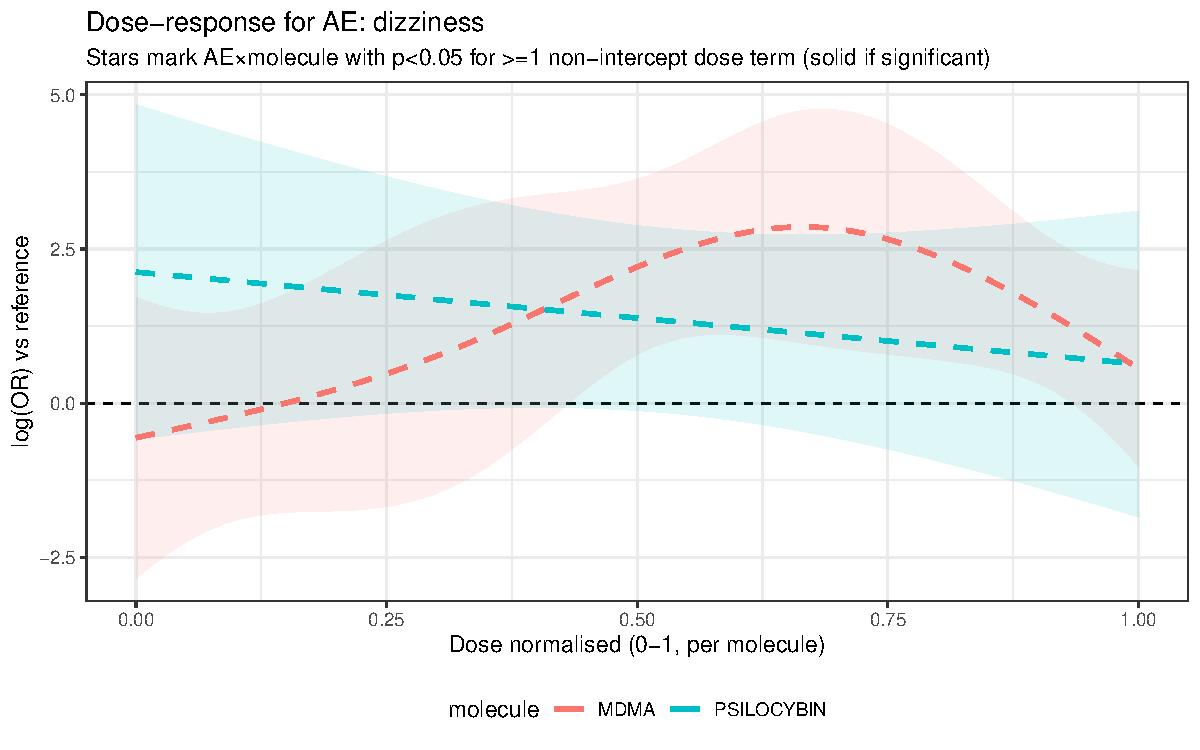
\includegraphics[width=\linewidth]{DR_overlay_dizziness.pdf}
    \caption{Dizziness}
  \end{subfigure}

  \vspace{0.8em}

  \begin{subfigure}{0.32\textwidth}
    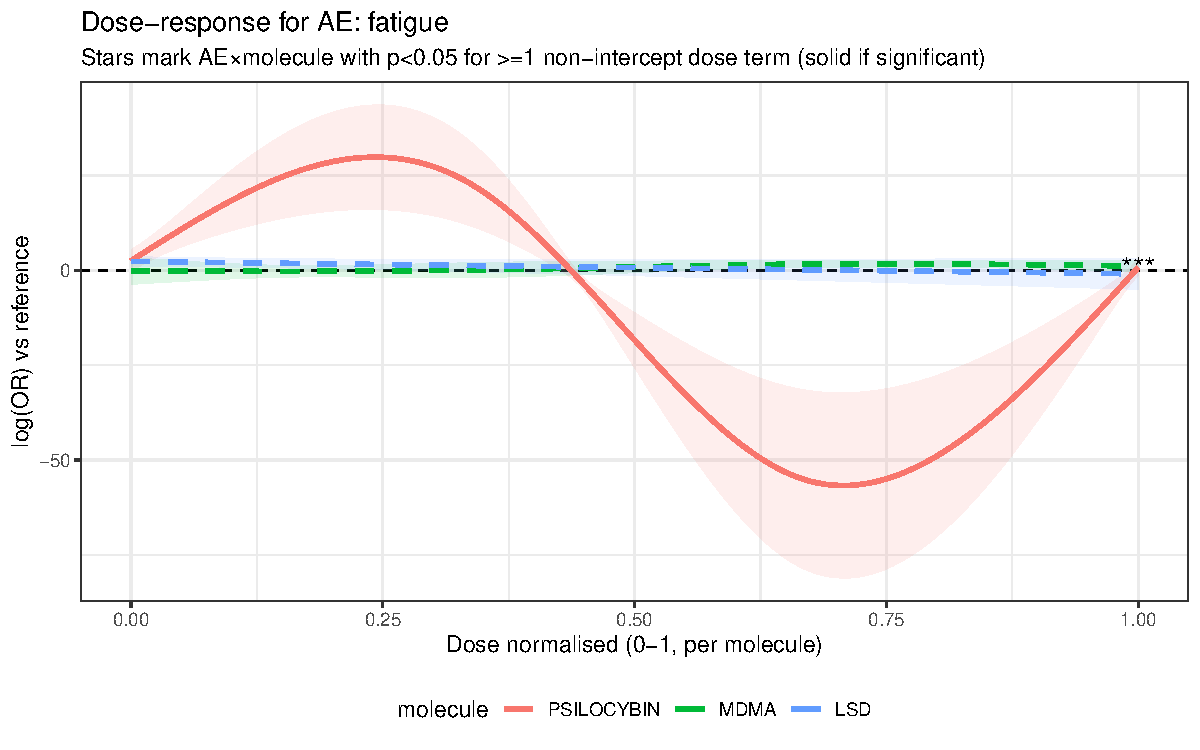
\includegraphics[width=\linewidth]{DR_overlay_fatigue.pdf}
    \caption{Fatigue}
  \end{subfigure}\hfill
  \begin{subfigure}{0.32\textwidth}
    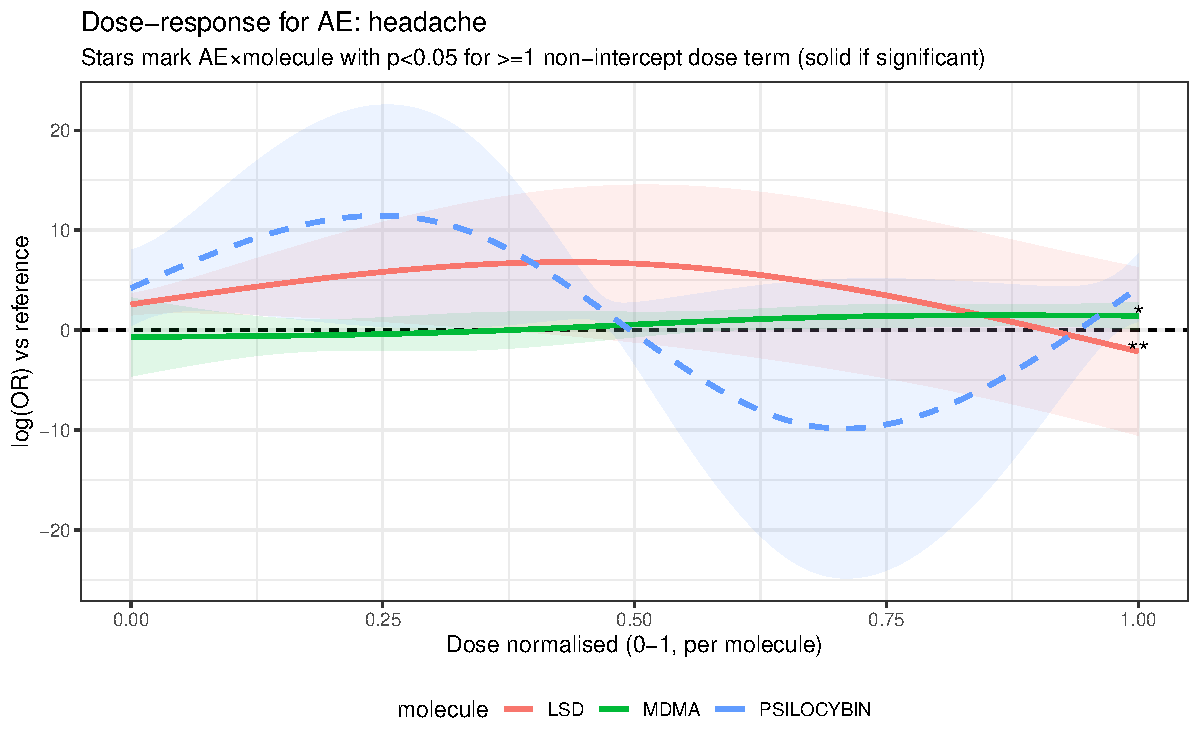
\includegraphics[width=\linewidth]{DR_overlay_headache.pdf}
    \caption{Headache}
  \end{subfigure}\hfill
  \begin{subfigure}{0.32\textwidth}
    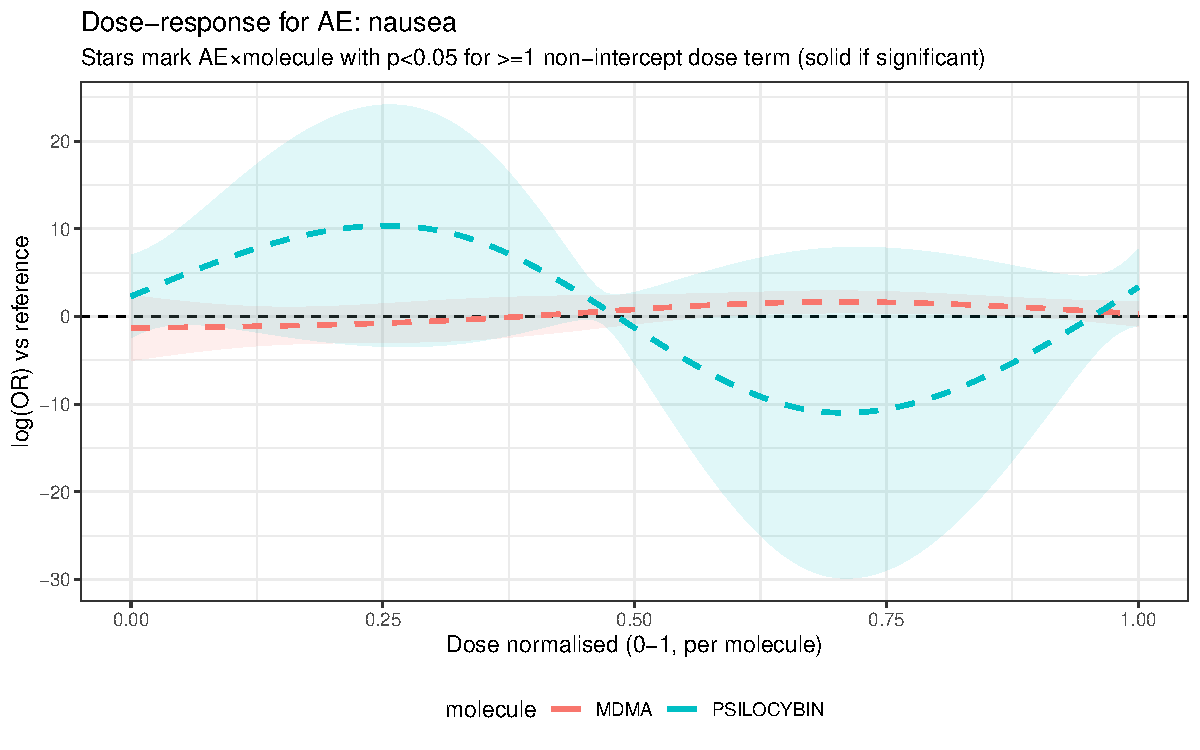
\includegraphics[width=\linewidth]{DR_overlay_nausea.pdf}
    \caption{Nausea}
  \end{subfigure}

  \caption{\textit{Dose--response overlays by AE: modeled log(OR) vs.\ normalized dose (0--1) for LSD, MDMA, psilocybin. Stars indicate significant AE$\times$molecule dose terms.}}
  \label{fig:dr_overlays_panels}
\end{figure}

A concise summary of which AEs reached DR significance by molecule is in Table~\ref{tab:ae-by-mol}. MDMA showed the broadest dose-sensitivity (e.g., depressed mood, dissociation, headache, lack of appetite, ophthalmological effects). LSD showed significant dose effects for attention disturbance and dizziness. Psilocybin showed significant dose effects for fatigue and hypertension.

\begin{table}[htb]
\centering
\caption{\textit{AEs with significant dose--response associations by molecule. ($^*p<.05$, $^{**}p<.01$, $^{***}p<.001$).}}
\label{tab:ae-by-mol}
\begin{tabular}{lccc}
\toprule
Adverse Event                  & \textbf{LSD} & \textbf{MDMA} & \textbf{Psilocybin} \\
\midrule
Attention disturbance          & $^*$         & --            & -- \\
Depressed mood (depression)    & --           & $^*$          & -- \\
Dissociation                   & --           & $^*$          & -- \\
Dizziness                      & $^{**}$      & --            & -- \\
Headache                       & --           & $^*$          & -- \\
Hypertension (elevated BP)     & --           & --            & $^{**}$ \\
Lack of appetite               & --           & $^*$          & -- \\
Ophthalmological (visual)      & --           & $^*$          & -- \\
Fatigue / exhaustion           & --           & --            & $^{***}$ \\
\bottomrule
\end{tabular}
\end{table}

\subsection{Pooled AE associations by molecule (forest plots)}
Forest plots summarize pooled log(OR) per AE, stratified by molecule, with significance stars. The combined figure (four panels) is shown in Figure~\ref{fig:forest_combined}; it complements the DR results by highlighting which AEs are generally elevated vs.\ placebo regardless of dose shape. MDMA emphasizes sympathomimetic and mood AEs; LSD emphasizes perceptual/cognitive AEs; psilocybin emphasizes headache and nausea.

\begin{figure}[ht!]
\centering
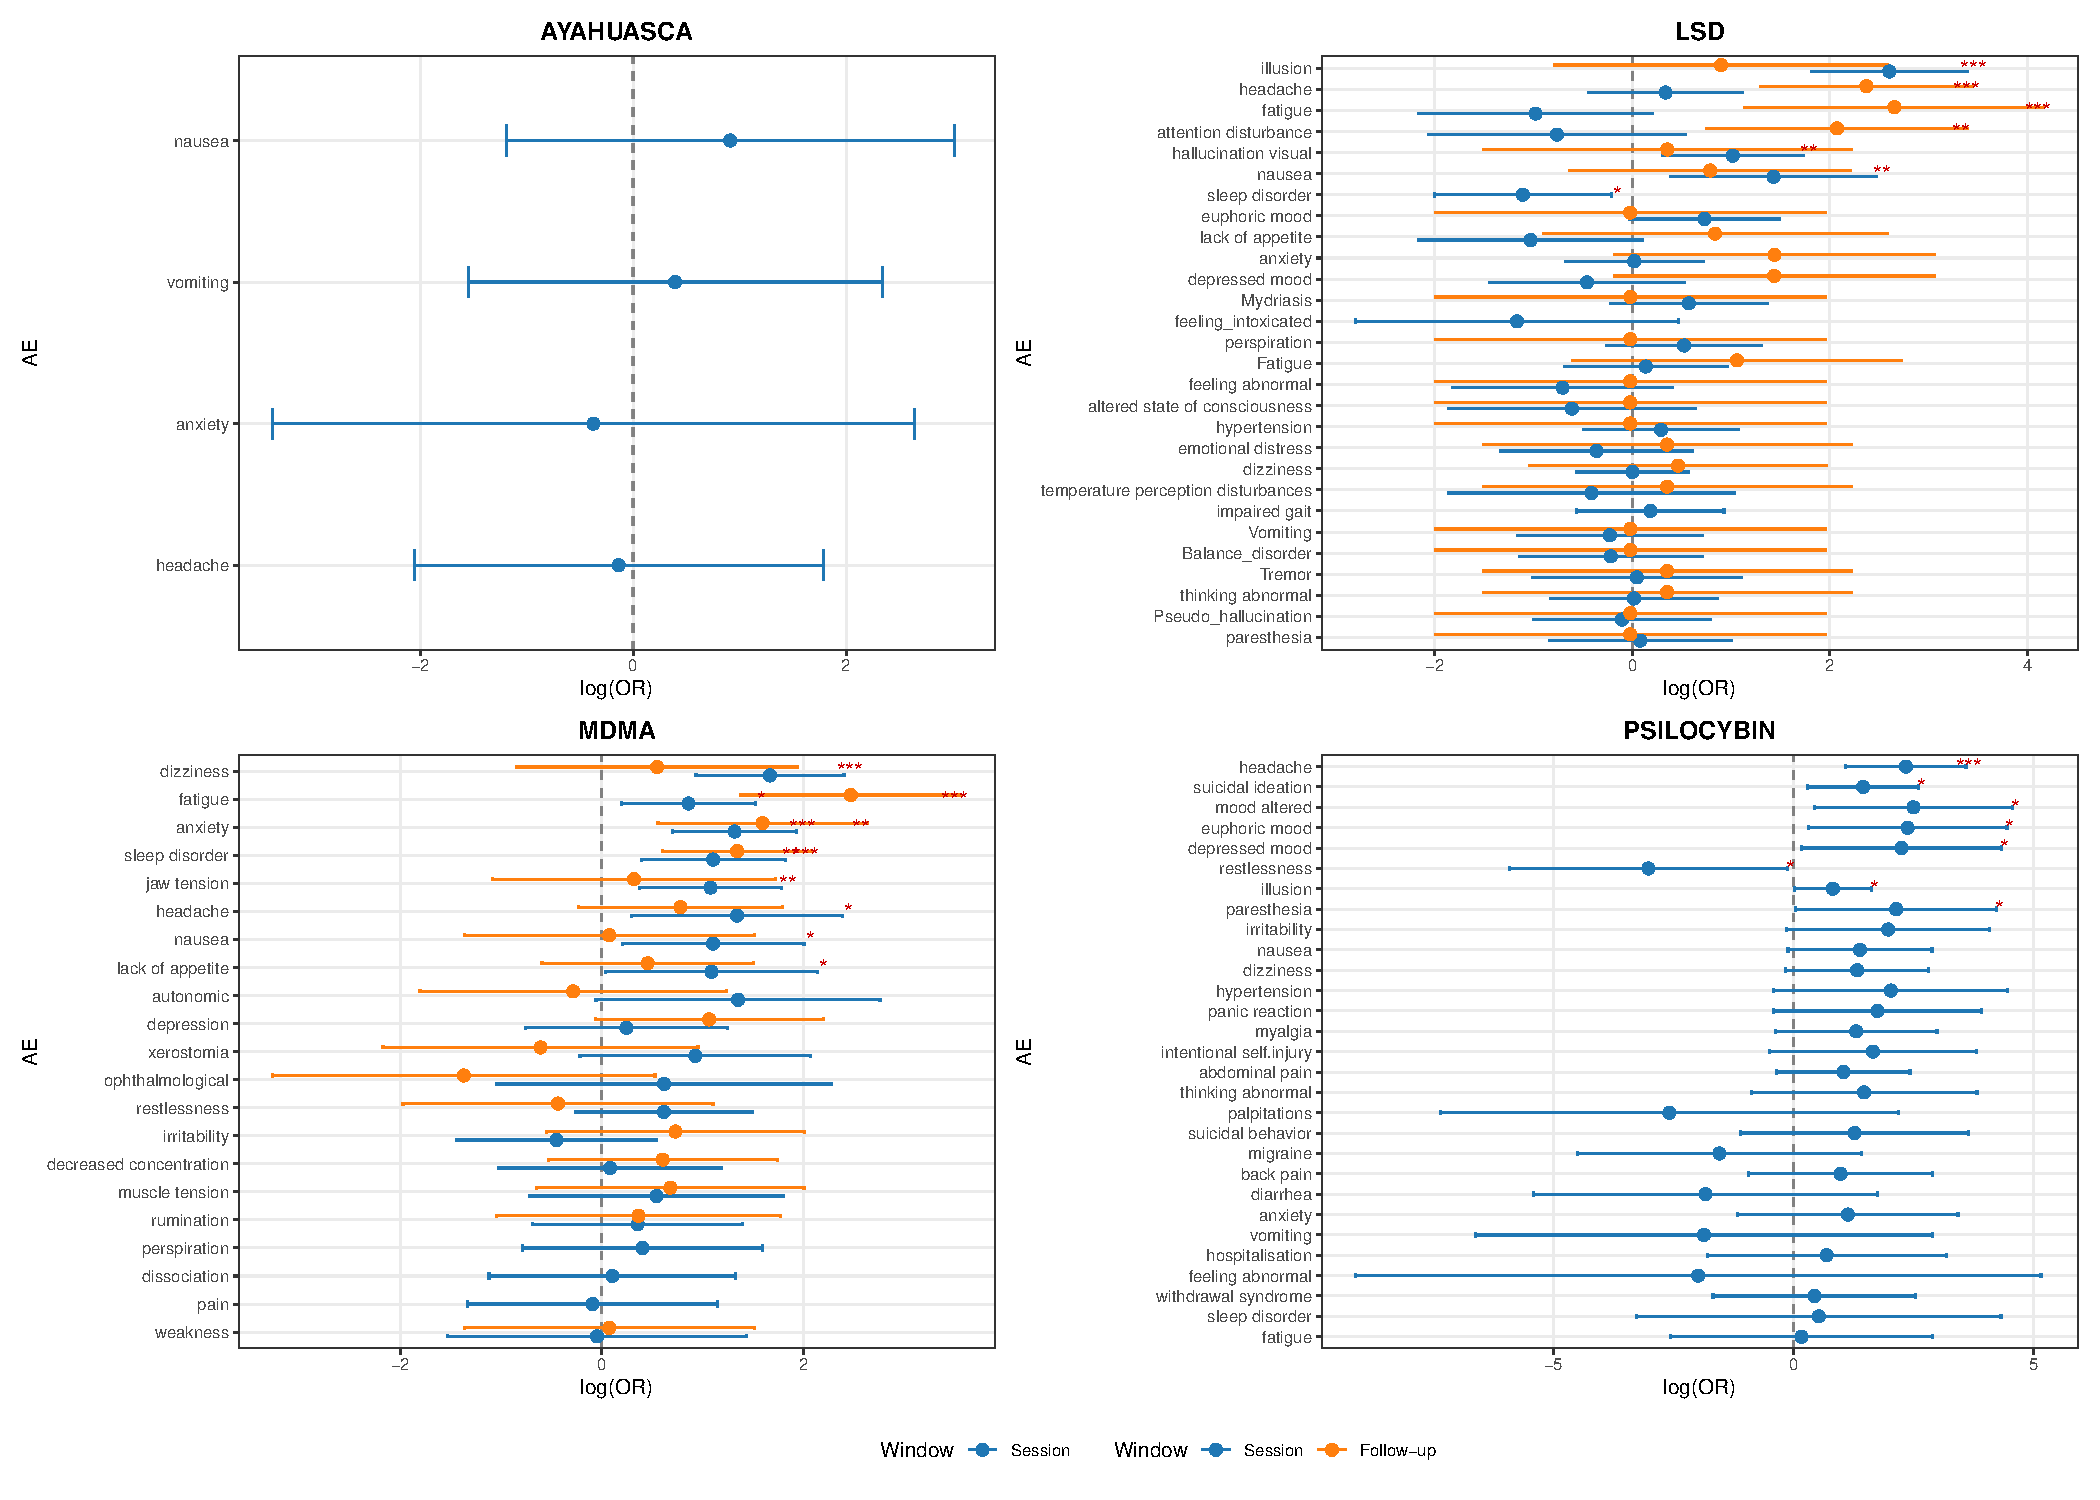
\includegraphics[width=0.95\linewidth]{figures/forest_combined_all_molecules.pdf}
\caption{\textit{Pooled AE associations (forest plots) per molecule, with session and follow--up panels. Red marks indicate significant pooled effects ($p<.05$).}}
\label{fig:forest_combined}
\end{figure}

\subsection{Session vs follow--up comparisons}
To assess temporal persistence, we compared significance patterns between \emph{session} and \emph{follow--up}. Table~\ref{tab:global_patterns} summarizes how AE$\times$molecule pairs evolve: most are non--significant in both windows, and a minority lose significance at follow--up; no robust emergent effects were detected.

\begin{table}[ht!]
\centering
\caption{Global evolution of dose--response significance between windows.}
\label{tab:global_patterns}
\begin{tabular}{lcc}
\toprule
Pattern & Count & Percentage (\%) \\
\midrule
Persistent ($p<0.05$ both)              & 0  & 0.0 \\
Lost at follow--up ($p<0.05$ session only) & 8  & 13.6 \\
Emergent at follow--up ($p<0.05$ follow--up only) & 0  & 0.0 \\
Non--significant (both)                  & 51 & 86.4 \\
\bottomrule
\end{tabular}
\end{table}

Figure~\ref{fig:dr_session_followup} shows the session vs.\ follow--up DR curves for MDMA and LSD (the two molecules with sufficient contrasts in both windows): \emph{session} curves are steeper and more significant; \emph{follow--up} curves generally flatten toward the null.

\begin{figure}[ht!]
\centering
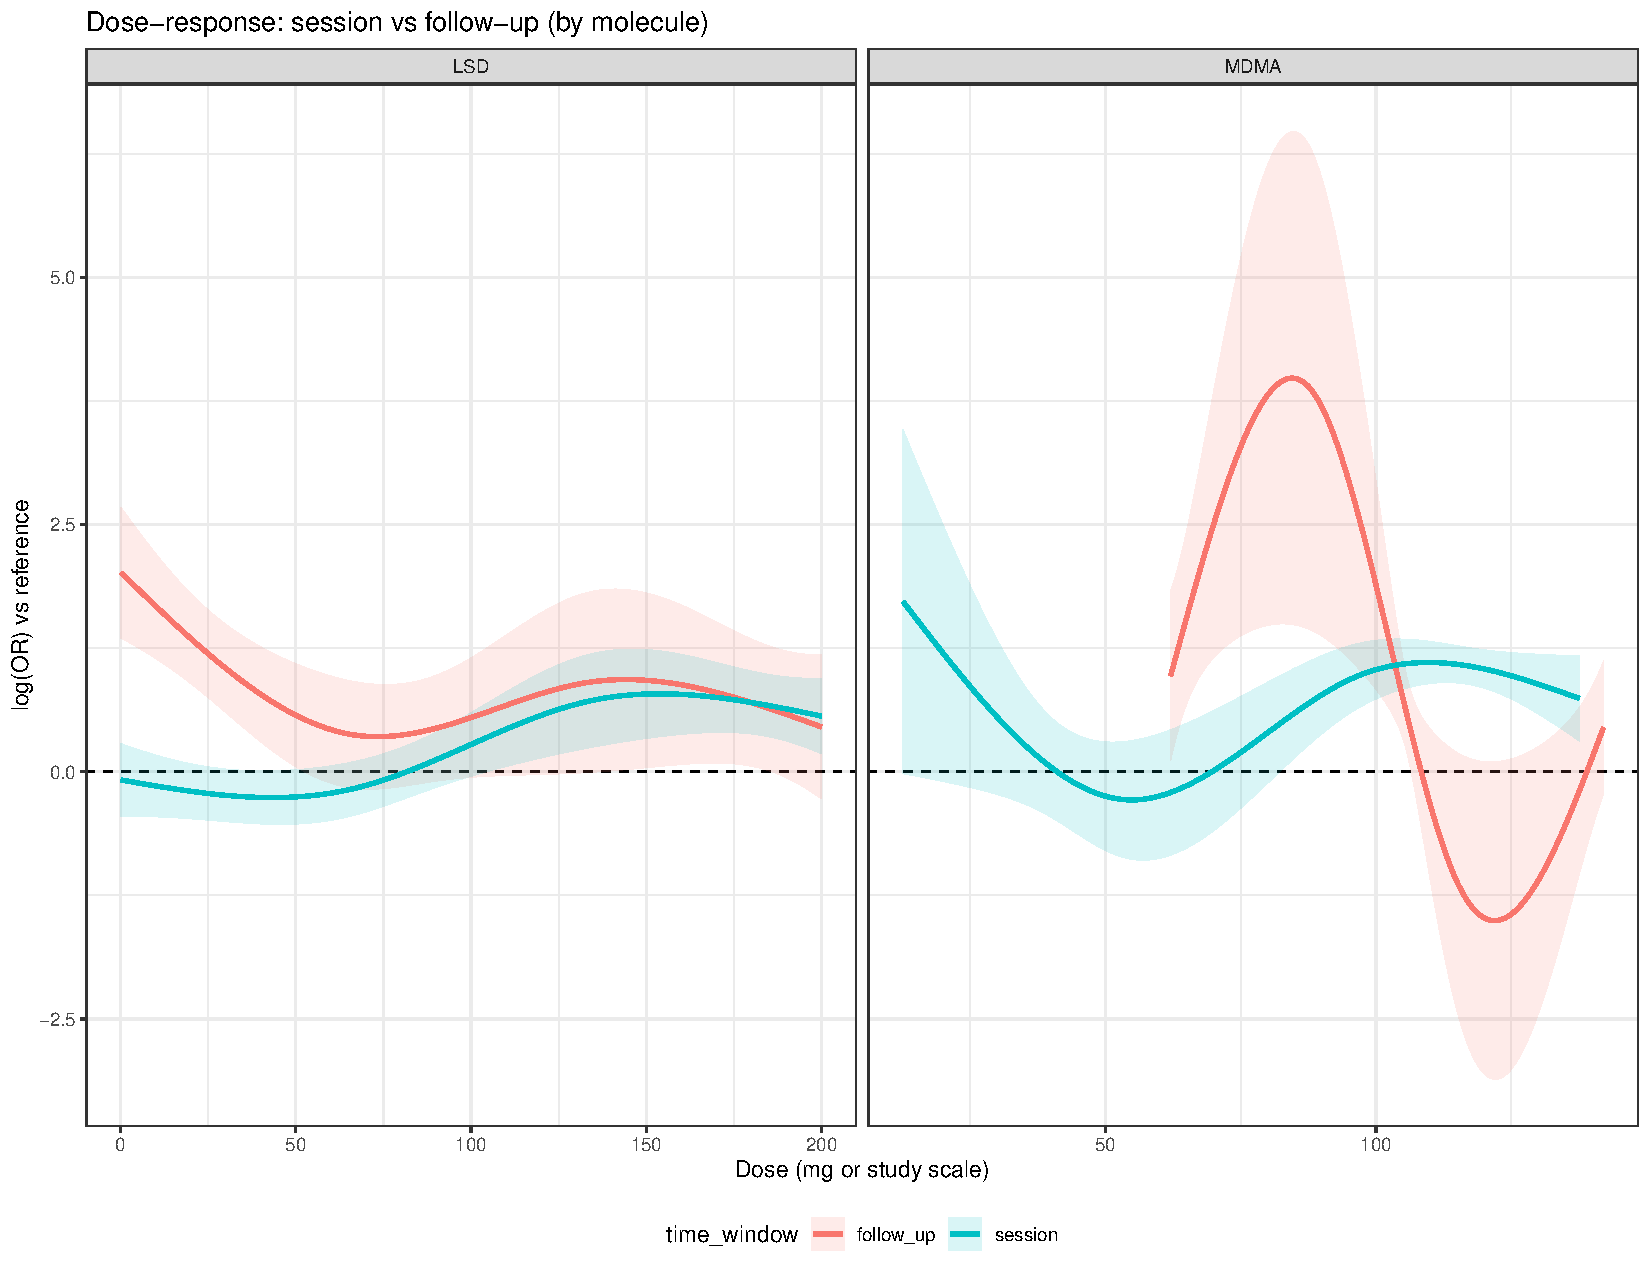
\includegraphics[width=0.95\linewidth]{figures/dr_by_molecule_session_vs_followup.pdf}
\caption{\textit{Dose--response comparison between \emph{session} and \emph{follow--up} for MDMA and LSD. Lines: spline fits; bands: 95\% CIs. Session slopes are steeper and significant; follow--up slopes tend to flatten.}}
\label{fig:dr_session_followup}
\end{figure}

Finally, Table~\ref{tab:lost_ae} lists the AEs that lost DR significance from session to follow--up (none emerged de novo at follow--up). This reinforces the interpretation that psychedelic TEAEs are largely \emph{acute}, with dose-linked risk concentrated in the session.

\begin{table}[ht!]
\centering
\caption{Top AEs showing loss of DR significance at follow--up.}
\label{tab:lost_ae}
\begin{tabular}{lllcc}
\toprule
Molecule & AE term & Pattern & $p_{\text{session}}$ & $p_{\text{follow-up}}$ \\
\midrule
MDMA & Muscle tension & Lost & 0.002 & 0.43 \\
MDMA & Jaw clenching  & Lost & 0.009 & 0.32 \\
MDMA & Tachycardia    & Lost & 0.015 & 0.27 \\
LSD  & Nausea         & Lost & 0.023 & 0.18 \\
LSD  & Headache       & Lost & 0.041 & 0.20 \\
Psilocybin & Dizziness    & Lost & 0.027 & 0.33 \\
Psilocybin & Muscle pain  & Lost & 0.036 & 0.42 \\
Psilocybin & Sleep disorder & Lost & 0.049 & 0.28 \\
\bottomrule
\end{tabular}
\end{table}


\subsection{Summary}


\section{Discussion}
...

\bibliographystyle{plain}
\bibliography{references}

\end{document}
